%file included in thesis.tex


\chapter{Sensors}
\label{chap3-sensors}

\section{2D Sensors}

\subsection{Laser Range Finder}


\subsubsection{Noise- and Error Sources}



\section{3D Sensors}
There are many different depth sensors available at the consumer market. This section will
outline some of them, and describe the \emph{MESA Imagining} SR-3000 in more detail.
The development of depth-sensing cameras and devices have accelerated the last years
because of the increased computational ability and the fact that electronics become
cheaper and cheaper. \cite{low-cost-depthcameras}

During the next years the video game industry most certainly will
incorporate this new technology into video games to take the games to a new level, such as
Microsofts \emph{Project Natal} for Xbox 360 \cite{project-natal}. This uses infrared
projected light stereo. The camera will sense depth by using stereo cameras to sense a
coded near-infrared light pattern, by using standard CMOS image sensors. According to
Microsoft the accuracy in depth will be about 1 cm, and practical ranges will be about
1 to 3.5 meters. The camera will operate at 640x480 pixel resolution at 60 Hz
\cite{conceivably-tech}.





\subsection{Stereo Camera}


\subsubsection{Camera Calibration}
To work with stereo images the captured images need to be rectified, i.e. the images need
to be corrected for distortion introduced by the camera lenses. This is a part of
calibrating the camera, meaning that the intrinsic parameters of the camera are
determined. That is distortion coefficients, and other camera parameters. 

Figure \ref{cahp3:fig-lensdist} below shows how the camera lenses of the Stereo camera distorts the pictures
towards the edges of the lens. 

\begin{figure}[htbp]
    \centering
   % \includegraphics[width=0.8\textwidth]{pics/left-rigth-camera-dist}
    \caption{The left and right camera distortion due to lens nonlinearities}
    \label{chap3:fig-lensdist}
\end{figure}

This distortion can be removed and are called rectifying the image. This makes common
features in the two images aligned horizontally. This makes it much easier for the matching
algorithm because it only need to match vertically.


\subsubsection{Depth resolution}
The depth resolution which can be expected from the Stereo cam are,
\begin{equation}
    \Delta Z = \frac{Z^2}{f T}\Delta d
\end{equation}
where $\Delta d$ is the smallest increment in disparity, $f$ is the focal distance, and
$T$ is the baseline.


\subsubsection{Noise- and Error Sources}




\subsection{Time-of-Flight Camera}
The time of flight camera gives out either Cartesian coordinates or intensity. This
intensity is the amplitude of the returned laser light. Figure
\ref{chap3:fig-tof-amppicture} shows a typical amplitude plot of the inside of a pipe.
\begin{figure}[htbp]
    \centering
   % 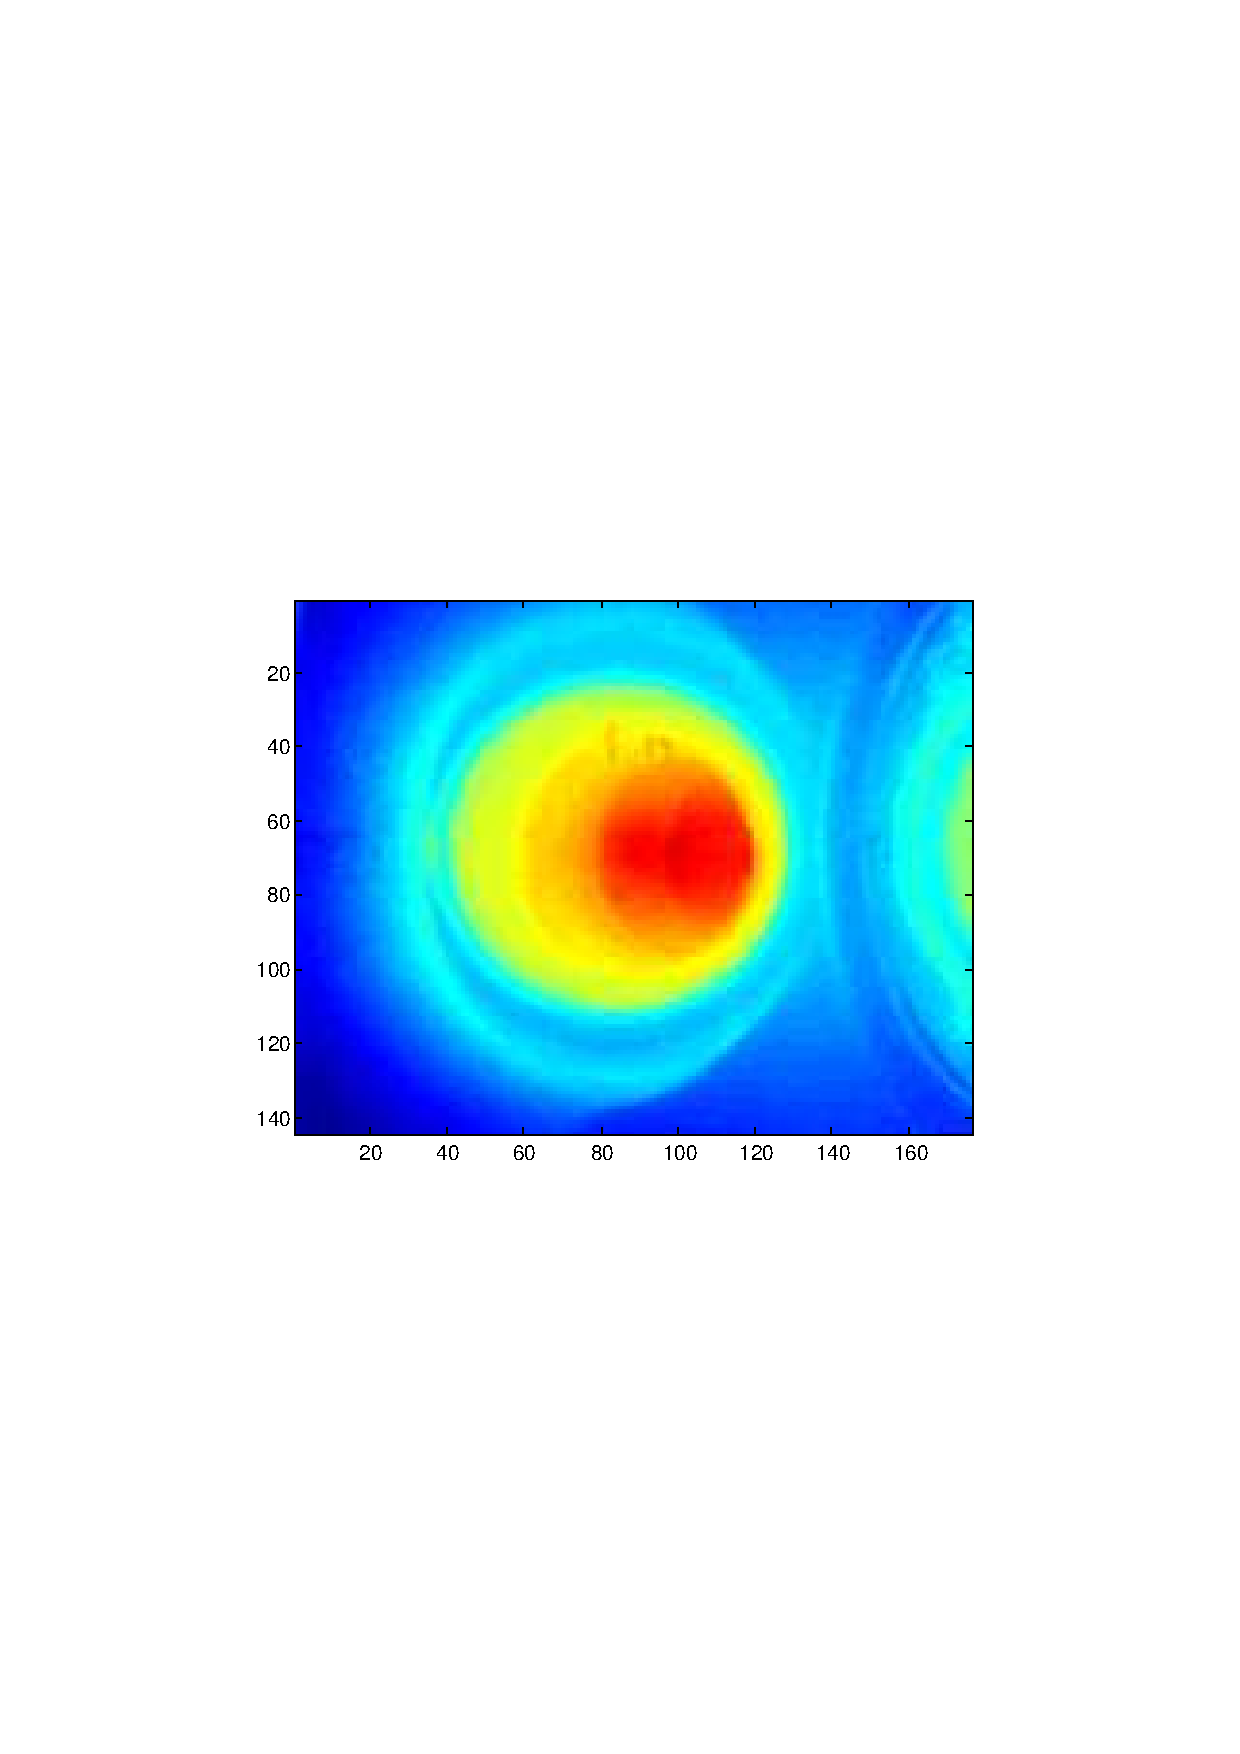
\includegraphics[width=0.8\textwidth]{pics/tof-amppicture}
    \caption{Typical amplitude image of the SR-3000 ToF-camera}
    \label{chap3:fig-tof-amppicture}
\end{figure}



\subsubsection{Noise- and Error Sources}
*******LIST THE ERROR SOURCES AND HOW TO SUPPRESS THEM**********




\section{Comparisons Between the Proposed Sensors}
\begin{table}[htbp]
    \centering
    \begin{tabular}{|c|c|c|c|c|c|c|c|c|}
        \hline
        Sensor & Range & Accuracy & FoV & Ang Res & Weight & Scan Freq & Power Cons &  Cost \\
        \hline
        LMS-100 & 20 m & 12 mm &  $270^{\circ}$ & $0.25-0.5^{\circ}$  & 1.1 kg    & 50 Hz & Not specified  & \$5500 \\
        \hline
        LMS-200 & 80 m & 30 mm &  $180^{\circ}$  & $0.25-1^{\circ}$  & 4.5 kg    & 75 Hz & Not specified &  \$5000 \\
        \hline
        UTM-30LX & 30 m & 30 mm & $270^{\circ}$ & $0.25^{\circ}$  & 210 g     & 40 Hz  &$<8$ W   &  \$5000 \\
        \hline
        URG-04LX & 4 m & 10 mm & $240^{\circ}$ & $0.36^{\circ}$ & 160 g  & 10 Hz & ca 2.5 W &  \$2400 \\
        \hline
        URG-04LX-URG01 & 5.6 m & 30 mm & $240^{\circ}$ & $0.36^{\circ}$ & 160 g & 10 Hz & ca 2.5 W & \$1100 \\
        \hline
        SR3000-ToF Camera & 7.5 m & 30 mm & $47.5$ x $ 39.6 ^\circ$ & 176 x 144 & -  & 25
        fps & 18 W max & \$10000 \\
        \hline
    \end{tabular}
    \caption{Comparison between the proposed sensors}
    \label{tab-chap3-sensors}
\end{table}
***FIX TABLE \ref{tab-chap3-sensors}********


\section{Sensor Configurations}
There are a couple of possible sensor configurations available for this project. ***SHOULD
MAYBE BE IN THE IMPLEMENTATION CHAPTER?****

The Laser Range Finder should alway be used in every sensor configuration. This should be
the primary source of length measurements since this is the most accurate of all the range
devices. 

The stereo camera might be looked upon as a cheap type of the Time-of-Flight camera. So
the two possible configurations are:
\begin{itemize}
    \item Laser Range Finder and Stereo Camera
    \item Laser Range Finder and Time-of-Flight Camera
\end{itemize}
The Stereo Camera will give sparse range data, while the Time-of-Flight camera will give
dense range data. 




